\documentclass[10pt,executivepaper]{article}
\usepackage[utf8]{inputenc}
\usepackage[spanish]{babel}
\usepackage{amsmath}
\usepackage{amsfonts}
\usepackage{amssymb}
\usepackage{graphics}
\usepackage{graphicx}
\usepackage[left=2cm,right=2cm,top=2cm,bottom=2cm]{geometry}
\usepackage{imakeidx}
\makeindex[columns=3, title=Alphabetical Index, intoc]
\usepackage{listings}
\usepackage{xcolor}
\usepackage{multicol}
\usepackage{changepage}
\usepackage{float}
\usepackage{cite}
\usepackage{url}

\definecolor{codegreen}{rgb}{0,0.6,0}
\definecolor{codegray}{rgb}{0.5,0.5,0.5}
\definecolor{codepurple}{rgb}{0.58,0,0.82}
\definecolor{backcolour}{rgb}{0.95,0.95,0.92}

\lstdefinestyle{mystyle}{
    backgroundcolor=\color{backcolour},
    commentstyle=\color{codegreen},
    keywordstyle=\color{magenta},
    numberstyle=\tiny\color{codegray},
    stringstyle=\color{codepurple},
    basicstyle=\ttfamily\footnotesize,
    breakatwhitespace=false,
    breaklines=true,
    captionpos=b,
    keepspaces=true,
    numbers=left,
    numbersep=5pt,
    showspaces=false,
    showstringspaces=false,
    showtabs=false,
    tabsize=3
}

\lstset{style=mystyle}

\title{Diferential Ecuation}

\author{A cargo del profesor: Luis Moctezuma Cervantes\\Escrito por: Adrian González Pardo}

\date{\today}

\newcommand\tab[1][1cm]{\hspace*{#1}}

\begin{document}
% Portada
%encabezado
\begin{minipage}{0.4\textwidth}
	\begin{flushleft}
		
\includegraphics[scale = 0.05]{logoescom.png}
	\end{flushleft}
\end{minipage}
\begin{minipage}{0.51\textwidth}
	\begin{flushright}
		
\includegraphics[scale = 0.055]{logoipn.png}
	\end{flushright}
\end{minipage}
\begin{center}
	\par\vspace{0.5cm}{
		\huge\textbf{Instituto Politécnico Nacional \\*[0.20cm] Escuela Superior de Cómputo}
	}
	\par\vspace{1cm}{
		\large\textbf{
		{Ecuaciones Diferenciales\\Profesor: Luis Moctezuma Cervantes\\Grupo: 1CM6\\Adrian González Pardo\\Semestre: 18/02}}
	}
	\par\vspace{1cm}{
		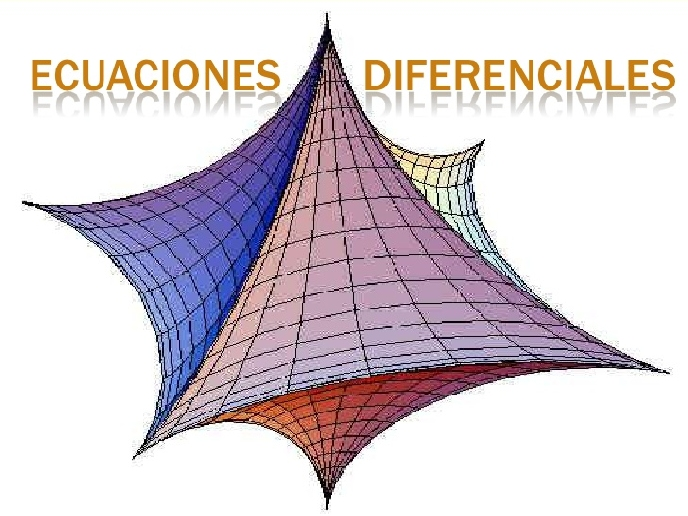
\includegraphics[scale=0.2]{ecuaciones.jpg}
	}
	\par\vspace{2cm}{
		Ultima fecha modificado: \today
	}
\end{center}

% Indice
\clearpage
\tableofcontents
\clearpage

%Contenido
\section{Introducción}
\subsection{Presentación}
Las ecuaciones diferenciales no son más que un conjunto de sistemas lineales o no lineales que representan modelo de comportamiento matemático, el cual puede ser aplicado en áreas como la ingeniería la cual puede servir para describir el comportamiento físico de un circuito electríco mediante las ecuaciones de voltaje de elementos lineales (resistencias, capacitadores e inductores), por otro lado igual puede ser aplicado en modelados matemáticos que puedan representar la medición estadística de una población de bacterias.\\
Ahora bien con el fin de facilitar el aprendizaje de estos temas se desarrollaran varias notas que se tomaron en el curso así como complemento de propía mano del escritor.
\subsection{Prerequisitos para la materia}
Si bien las matemáticas guardan una intima pero fuerte relación entre sus topicos es importante marcar algunos prerequisitos para poder dar seguimiento o poder tener un mejor entendimiento con la materia
\begin{center}
  \begin{tabular}{|p{5.5cm}|p{5.5cm}|}
    \hline
    Principios de Cálculo & Nociones de Algebra Lineal\\
    \hline
    Nociones de Análisis Vectorial & Nociones de Física\\
    \hline
  \end{tabular}
\end{center}
Si bien podriamos desglosar todos y cada uno de los prerequisitos de cada asignatura, no es la idea asustar a los pequeños lectores o consultores de este documento, ahora si continuemos

\subsection{Libros de consulta}
Si bien las ecuaciones diferenciales pueden ser estudiadas en cursos los cuales no soliciten libro, te puedes apoyar de material que se encuentra de forma gratuita pero quizas poco legal en internet, por ello yo no quiero alentarte a realizar una conducta dañina a los autores, mi mejor recomendación en este aspecto, es quizas consigue los pdf's pero después de ello busca la forma de conseguirlo en físico para tu formación o para el apoyo de tus compañeros o alumnos.
\begin{itemize}
  \item Dennis Zill, Ecuaciones Diferenciales $\rightarrow$ Para comenzar desde el inicio y sin complicaciones
  \item Editorial Trillas Canek, Ecuaciones Diferenciales ordinarias $\rightarrow$ Para subir el nivel con respecto al Dennis
  \item Makarenko, Problemas de Ecuaciones Diferenciales ordinarias 1996 $\rightarrow$ Para ejercicios bastante completos y extensos
\end{itemize}

\section{Inicio}
Recordemos que para tener un buen inicio con respecto al curso es necesario tener un ligero repaso a las Técnicas de Integración.
\subsection{Técnicas de Integración}
Las técnicas de integración son herramientas que nos seran de utilidad como si fuese la frase celebre o la bendición del día a día.\\
Recordemos que las técnicas más comunes que tenemos son 4:
\begin{enumerate}
  \item Por sustitución
  \item Por partes
  \item Por sustitución trigonometrica
  \item Por fracciones parciales
\end{enumerate}
Ahora con esto, comencemos.
\subsubsection{Por sustitución}
\textbf{Teorema:} Sea $g(x)$ una función derivable y supongase que $F(x)$ es una antiderivada de $f(x)$.\\
Entonces si $u=g(x)$ tenemos lo siguiente:\\
\[\int f(g(x))g^{l}(x)dx = \int f(u)du = F(u) + C = F(g(x)) + C   \colon C \in \mathbb{R}\]
\\
\textbf{Ejemplos:}
\\
\[\int \frac{x}{\cos^{2}(x^{2})}dx\]
\textit{Solución}\\
Recordemos identidades trigonométrica como lo es: $\frac{1}{\cos(x)}=\sec(x)$, entonces tenemos lo siguiente
\[\int x \sec^{2}(x^2)dx\]\\
Ahora por sustitución definimos a $u=x^{2} \rightarrow du=2x dx$ completando la integral tenemos:
\[\frac{1}{2}\int \sec^{2}(u)du = \frac{1}{2}\tan(u) + C\]\\
Sustituyendo los valores de $u$ tenemos la integral resuelta:
\[\int \frac{x}{\cos^{2}(x^{2})} = \frac{1}{2} \tan(x^{2}) + C \]
\vspace{1.5cm}
\[\int \frac{3}{\sqrt{5-9x^{2}}}dx\]
\textit{Solución}\\
Recordemos la forma de las integrales que pasan a la forma inversa de una función trigonométrica (arcos) podemos pensar en el cambio de variable por $u=3x \rightarrow du=3dx$, entonces tendremos lo siguiente:\\
\[\int \frac{1}{\sqrt{5-u^{2}}}du = \arcsen(\frac{u}{5}) + C\]\\
Sustituyendo $u$ por el valor que tenemos en $x$ tenemos:\\
\[\int \frac{3}{\sqrt{5-9x^{2}}}dx = \arcsen(\frac{3x}{5}) + C\]
\vspace{1.5cm}
\clearpage
\[\int \frac{6 e^{\frac{1}{x}}}{x^{2}}dx\]\\
\textit{Solución}\\
Para este tipo de integral lo que podemos hacer es proponer el siguiente cambio de variable $u = \frac{1}{x} \rightarrow du=-\frac{1}{x^{2}}dx$\\
\[-6\int e^{u}du = -6 e^{u} + C \]\\
Sustituyendo $u$ por su valor con respecto a $x$ tenemos:\\
\[\int \frac{6 e^{\frac{1}{x}}}{x^{2}}dx=-6 e^{\frac{1}{x}} + C\]

\vspace{1cm}
\[\int\frac{e^{x}}{4 + 9 e^{2x}}dx\]
\\
\textit{Solución:}\\
Se propone el siguiente cambio de variable $u=3e^{x}\rightarrow du= 3e^{x}dx$\\
\[\frac{1}{3}\int \frac{1}{4+u^{2}}du=\frac{1}{6}\arctan{\frac{u}{2}}+C\]
\\Sustituyendo los valores de $u$ con respecto a $x$\\
\[\int\frac{e^{x}}{4 + 9 e^{2x}}dx = \frac{1}{6}\arctan{\frac{3e^{x}}{2}}+C\]\\
\textbf{Ejecicio propuesto:}\\
\begin{enumerate}
  \item \[\int \frac{a^{\tan(t)}}{\cos^{2}(t)}dt\]
  \textbf{Hint:} No te espantes y sustituye ese $\frac{1}{cos^{2}(x)}$ por su identidad trigonométrica correspodiente.
\end{enumerate}


\clearpage
\subsubsection{Por partes}
\textbf{Definición:} Sea un función dada por el producto de dos funciones cuya función se desea buscar su integral indefinida, la formula esta dada por:\\
\[\int u dv = uv - \int vdu\]\\
\emph{Algunos tipos a la hora de aplicar la regla de la integración por partes tenemos que tomar encuenta que la aplicación va acorde a la presedencia de sus funciones}
\begin{itemize}
  \item Recordemos la famosa regla ILATE que nos ayuda a definir la prioridad de $u$
  \item I es aplicado para las funciones inversas
  \item L es aplicado para aquellas funciones logarítmicas
  \item A es aplicado a todas esas funciones algebraicas
  \item T es aplicado a todas las funciones trigonométricas
  \item E es aplicado a todas las funciones que sean exponenciales
\end{itemize}
Dicho esto continuemos\\
\textbf{Ejemplos:}\\
\[\int \arcsen(x)dx\]\\
\textit{Solución}\\
Por lo cual aplicamos las reglas y sabemos que hay una función inversa con respecto a la función inversa del $\sen(x)$ por lo que proponemos a $u=\arcsen(x)\rightarrow du = \frac{1}{\sqrt{1-x^{2}}}dx$ \& $dv=dx \rightarrow v=x$
\\
\[x\arcsen(x)-\int \frac{x}{\sqrt{1-x^{2}}}dx\]\\
Resolviendo la ultima integral haciendo cambio de variable $w=1-x^{2} \rightarrow dw=-2x dx$\\
\[x\arcsen(x)-\int \frac{1}{\sqrt{w}}dw \Leftrightarrow x\arcsen(x)+\frac{1}{2}\sqrt{w} + C\]
Sustituyendo $w$ con su valor de x tenemos:
\[\int \arcsen(x)dx=x\arcsen(x)+\frac{1}{2}\sqrt{1-x^{2}}+C\]
\vspace{1cm}
\[\int t^{6}\ln(t)dt\]\\
\textit{Solución}\\
De acuerdo a lo que tenemos aquí y a las reglas sabemos, tendremos lo siguiente $u=\ln(t) \rightarrow du=\frac{1}{t}dt$ \& $dv=t^{6}dt \rightarrow v=\frac{t^7}{7}$\\
\[\frac{t^7}{7}\ln(t)-\frac{1}{7}\int t^{6}dt\]
Ahora resolviendo la ultima integral tenemos que la resolución es:\\
\[\int t^{6}\ln(t)dt = \frac{t^{7}}{7}-\frac{t^{7}}{49} + C\]
\vspace{1cm}
\[\int t^{n}\ln(t)dt \colon n \in \mathbb{N}\]
\textit{Solución}\\
Aplicando la regla ILATE tenemos lo siguiente: $u=\ln(t)\rightarrow du=\frac{1}{t}dt$ \& $dv=t^{n}dt \rightarrow v=\frac{t^{n+1}}{n+1}$, ahora aplicando la regla tenemos:\\
\[\frac{t^{n+1}}{n+1}\ln(t)-\frac{1}{n+1}\int t^{n}dt\]
Ahora solo solucionamos la ultima integral:
\[\int t^{n}\ln(t)dt = \frac{t^{n+1}}{n+1}\ln(t)-\frac{t^{n+1}}{(n+1)^{2}} + C \colon \forall n \in \mathbb{N}\]
\vspace{1cm}
\[\int e^{x}\sin(x)dx\]\\
De esta integral partiremos de dos soluciones distintas ambas llegando al mismo resultado:\\
\textit{Solución 1:}\\
Tomaremos esta integral de forma directa de tal forma que tendremos lo siguiente $u=\sin(x)\rightarrow du= \cos(x)dx$ \& $dv=e^{x}dx \rightarrow v=e^{x}$, aunado a esto tenemos:
\[e^{x}\sin(x) - \int e^{x}cos(x)dx \]
Volveremos a aplicar la regla de la integral por parte esta vez modificando las letras para hacerlo un poco más explicito $u=a$ \& $v=b$, por lo que tendremos es $a=cos(x) \rightarrow da=-sin(x)dx$ \& $db=e^{x}dx \rightarrow b=e^{x}$, ahora continuando el desarrollo de la integral tendremos:
\[e^{x}\sin(x)-\{e^{x}\cos(x)+\int e^{x}\sin(x)dx\}\]
Ahora aplicando distribución y signos tenemos:
\[e^{x}\sin(x)-e^{x}\cos(x)-\int e^{x}\sin(x)dx\]
Como podemos ver esto se trata de la misma integral a la que tenemos originalmente, lo que nos permite concluir que se trata de una integral ciclica, por lo tanto lo que haremos es lo siguiente:
\[\int e^{x}\sin(x)dx = e^{x}\sin(x)-e^{x}\cos(x)-\int e^{x}\sin(x)dx\]
Algebraicamente haremos que la integral del lado derecho pase del lado izquierdo:
\[2\int e^{x}\sin(x)dx = e^{x}\sin(x)-e^{x}\cos(x)\]
Ahora por simple algebra:
\[\int e^{x}\sin(x)dx = \frac{1}{2}\{e^{x}\sin(x)-e^{x}\cos(x)\}+C\]

\textit{Solución 2:}\\
Veamos a $\sin(x)$ como su representación en el campo de los números complejos con ayuda de la identidad de Euler:
\[\sin(x)= \frac{1}{2i}(e^{ix}-e^{-ix})\]
Para complementar esto veamos igual al $\cos(x)$ en su forma de Euler:
\[\cos(x)= \frac{1}{2}(e^{ix}+e^{-ix})\]
Entonces tendremos:
\[\frac{1}{2i}\int e^{x}(e^{ix}-e^{-ix})dx \Leftrightarrow \frac{1}{2i}\{\int e^{x(1+i)} - \int e^{x(1-i)}\}\]
Por lo que propondremos el cambio de variable respectivo $u$ y $v$ donde $u=x(1+i)$ y $v=x(1-i)$, entonces sus derivadas con respecto a $x$ son $du=(1+i)dx$ y $dv=(1-i)dx$, entonces:
\[\frac{1}{2i}\{\frac{1}{1+i}e^{x(1+i)}-\frac{1}{1-i}e^{x(1-i)}\}+C\]
Ahora aplicaremos el complemento de cada fracción compleja por lo que en el resultado tendremos:
\[\frac{1}{2i}\{\frac{1+i}{2}e^{x(1+i)}-\frac{1-i}{2}e^{x(1-i)}\}+C\]
Ahora separando terminos del campo $\mathbb{R}$ y $\mathbb{C}$ tendremos:
\[\frac{1}{4i}\{e^{x(1+i)}-e^{x(1-i)} + i(e^{x(1+i)}+e^{x(1-i)})\}+C\]
Separando terminos y reordenando:
\[\frac{1}{4i}\{e^{x(1+i)}-e^{x(1-i)}\} + \frac{1}{4}\{(e^{x(1+i)}+e^{x(1-i)})\}+C\]
Factorizando todos los valores de $e^{x}$ tendremos:
\[\frac{e^{x}}{4i}\{e^{xi}-e^{-xi}\} + \frac{e^{x}}{4}\{(e^{xi}+e^{-xi})\}+C\]
Ahora aplicando identidad de Euler:
\[\frac{1}{2}e^{x}\sin(x) + \frac{1}{2}e^{x}\cos(x)+C\]
Reordenando todo:
\[\frac{1}{2i}\int e^{x}(e^{ix}-e^{-ix})dx \Leftrightarrow \frac{1}{2i}\{\int e^{x(1+i)} - \int e^{x(1-i)}\} = \frac{1}{2}e^x\{\sin(x)+\cos(x)\}+C\]
\clearpage
\[\int \sin^{n}(x)dx \colon \forall n\in\mathbb{N}\geq 2\]
\textit{Solución}\\
Reescribiremos la integral como:
\[\int \sin^{n-1}(x)\sin(x)dx\]
Ahora si podremos aplicar las reglas podemos considerar que $\sin^{n-1}(x)$ como un valor exponencial, por lo que propondremos lo siguiente, $u=\sin^{n-1}(x) \rightarrow du=(n-1)\sin^{n-2}(x)\cos(x)dx$ \& $dv = \sin(x)dx \rightarrow v=-\cos(x)$, ahora:
\[-\cos(x)\sin^{n-1}(x) + (n-1)\int \sin^{n-2}(x)\cos^{2}(x)dx\]
Recordemos las identidades trigonométricas de valores que son iguales a $1$:
\[1=\cos^2(x)+\sin^{2}(x)\]
\[1=\sec^{2}(x)-\tan^{2}(x)\]
Aplicaremos esta identidad en la integral de tal forma que podremos sustituir la integral a dos partes:
\[-\cos(x)\sin^{n-1}(x) + (n-1)\{\int \sin^{n-2}(x)dx -\int\sin^{n}(x)dx\}\]
Aplicando distributividad:
\[\int\sin^{n}(x)dx=-\cos(x)\sin^{n-1}(x) + (n-1)\int \sin^{n-2}(x)dx -(n-1)\int\sin^{n}(x)dx\]
Ahora aplicando algebra:
\[n\int\sin^{n}(x)dx=-\cos(x)\sin^{n-1}(x) + (n-1)\int \sin^{n-2}(x)dx + C\]
De nuevo aplicando algebra:
\[\int\sin^{n}(x)dx=\frac{1}{n}\{-\cos(x)\sin^{n-1}(x) + (n-1)\int \sin^{n-2}(x)dx\} + C \colon \forall n\in\mathbb{N}\geq 2\]
\vspace{1cm}
\[\int \cos^{n}(x)dx \colon \forall n\in\mathbb{N}\geq 2\]
\textit{Solución:}\\
Ahora ya que tenemos noción de la integral anterior podemos proceder con lo siguiente:
\[\int\cos^{n-1}(x)\cos(x)dx\]
\[u=\cos^{n-1}(x)\rightarrow du=-\cos^{n-2}(x)\sin(x)dx\]
\[dv=\cos(x)dx \rightarrow v=\sin(x)\]
Esto implica:
\[\cos^{n-1}(x)\sin(x)+(n-1)\int\cos^{n-2}\sin^{2}(x)dx\]
Aplicando igual identidades trigonométrica directamente:
\[\cos^{n-1}(x)\sin(x)+(n-1)\{\int\cos^{n-2}(x)dx - \int\cos^{n}(x)dx\}\]
\[\int\cos^{n}(x)dx =\cos^{n-1}(x)\sin(x)+(n-1)\int\cos^{n-2}(x)dx-(n-1)\int\cos^{n}(x)dx\ \]
Ahora con algebra:
\[n\int\cos^{n}(x)dx =\cos^{n-1}(x)\sin(x)+(n-1)\int\cos^{n-2}(x)dx+C\]
\[\int\cos^{n}(x)dx =\frac{1}{n}\{\cos^{n-1}(x)\sin(x)+(n-1)\int\cos^{n-2}(x)dx\}+C \colon \forall n\in\mathbb{N}\geq 2\]
\textbf{Ejercicios propuestos:}
\begin{enumerate}
  \item \[\int\ln(t)dt\]
  \item \[\int \cos^{3}(x)dx\]
  \item \[\int \sin^{5}(x)dx\]
\end{enumerate}
\clearpage
\subsubsection{Integración trigonométrica}
Si bien ya aplicamos integración con funciones trigonométricas es importante tambien poder saber un par de tecnicas con respecto a propiedades de las mismas para que originen un ahorro de tiempo a la hora de resolver diversos ejercicios y/o resolver ecuaciones diferenciales.\\
\textbf{Tipo I:}
\[\int\sin^{n}(x)dx;\int\cos^{n}(x)dx\colon\forall n\in\mathbb{Z^{+}}\]
\textit{Podemos aplicar algunas propiedades como la propiedad de $1$ o en el caso de ser valores de $n$ impar podemos hacer lo siguiente:}
\[\sin^{2}(x)=\frac{1}{2}(1-\cos(2x))\]
\[\cos^{2}(x)=\frac{1}{2}(1+\cos(2x))\]
\[1=\cos^{2}(x)+\sin^{2}(x)\]
\[1=\sec^{2}(x)-\tan^{2}(x)\]
\textbf{Ejemplos}

\printindex
\end{document}
